\documentclass[UTF8]{ctexart}
\usepackage{amsmath}
\usepackage{amssymb}
\usepackage{booktabs}
\usepackage{background}
\usepackage{caption,subcaption}
\usepackage{CJKfntef}
\usepackage{cprotect}
\usepackage{enumitem}
\usepackage{fancyhdr}
\usepackage{float}
\usepackage{fontspec}
%\usepackage{fourier}
\usepackage{geometry}
\usepackage{listings}
\usepackage{tcolorbox}
\usepackage{tikz}
\usetikzlibrary{arrows.meta}
\usepackage{xcolor}

\geometry{a5paper, top=0.1cm, left=1cm, right=1cm, bottom=1cm, footskip=0.1cm}
\setCJKmainfont[BoldFont={汉仪文黑-85W},ItalicFont={方正苏新诗柳楷简体}]{汉仪文黑-55W}
\setfontfamily\Issue{Century Schoolbook}
\setfontfamily\Genshin{Genshin Teyvat Lingua Franca}
\newCJKfontfamily\TitleFont{思源宋体 CN Heavy}
\newfontfamily\timesnewroman{Times New Roman}
%\reversemarginpar

\pagestyle{fancy}
\fancyhf{}
\cfoot{\sffamily\footnotesize{-\ \thepage\ -}}
%\CTEXsetup[format = {\centering\bfseries\large}, beforeskip = 3pt, afterskip = 3pt]{section}

\colorlet{darkcyan}{cyan!50!black}
\newcommand\Black[1]{\textcolor[gray]{0.3}{#1}}
\newcommand\Brown[1]{\textcolor[HTML]{998A4E}{#1}}
\newcommand\Emph[1]{\colorbox{green!10}{\textcolor{green!30!black}{#1}}}
\newcommand\Notes[1]{\textcolor{yellow!50!black}{\small #1}}
\newcommand\Example[1]{\textcolor{cyan!70!black}{\small #1}}
\newcommand\keyword[1]{\textcolor{violet}{\textbf{\texttt{#1}}}}

\newtcolorbox{mybox}[1][其他规则]{colback=cyan!10, colframe=cyan, arc=1pt, title={#1}}

\renewcommand\d{\mathrm{d}}

\lstset{
    basicstyle=\small\ttfamily, %注意行末有逗号!
    keywordstyle=\bfseries\color{blue!70!black},
    commentstyle=\color{cyan!90!black},
    stringstyle=\color{green!40!black},
    columns=flexible,
    numbers=left,
    numberstyle=\footnotesize,
    escapechar=`,
    frame=shadowbox,
    %rulesepcolor=\color{red!20!blue!20!green!20}
    backgroundcolor=\color{cyan!5!white},
    language = C++,
    tabsize = 4,
    breaklines = true,
    showstringspaces = false,
}

\newcommand\IssueNumber{32}
\newcommand\Date{2024-6-20}
%\newcommand\Contributer{@金光日}
\newcommand\Subject{高级程序设计语言(Java)}


\begin{document}
\backgroundsetup{contents=
\includegraphics{上半示例.png}, center, scale=1, angle=0, opacity=1}
\BgThispage
\begin{center}
%{\scriptsize\Issue \textcolor[HTML]{C8BA83}{\Genshin WEEKLY TIPS}}
\phantom{...}

{\Large\textcolor{brown!40!white}{\makebox[10cm][s]{\Genshin WEEKLY KNOWLEDGE TIPS}}}

\vspace{-2em}

{\Huge\bfseries\TitleFont \Black{知\ 识\ 小\ 料}}


\vspace{-0.1cm}
{\footnotesize \Brown{「电计 2203 班」周常规知识整理共享}}
\end{center}

\vspace{-0.5cm}


\begin{figure}[H]
\hspace{1cm}
\begin{minipage}[t]{0.3\textwidth}
\centering
    \Brown{\Genshin ISSUE}

    \vspace{-0.6cm}
    \Huge \Issue\slshape\bfseries\Black{\IssueNumber}
\end{minipage}
\hfill
\begin{minipage}[t]{0.35\textwidth}
\centering
    \Brown{日期:\Date} \\
%\vspace{-0.1cm}
%    \Brown{贡献者:\Contributer} \\
\vspace{-0.1cm}
    \Brown{学科:\Subject} \\
\end{minipage}
\hspace{0.8cm}
\end{figure}

{\color{cyan!50!black}
Java 考试选手应知应会的 C++ 知识。
}

\section{类与对象·基本}
就像 Java 一样,C++ 也有类与对象的概念。类与对象的基本格式如下所示:

\begin{lstlisting}
class Person{
	private: //私有的成员变量
		char name[30];
		int age;
	public:
		Person(char newName[30], int newAge){ //公有的构造器
			strcpy(this->name, newName); //字符串复制需要string.h头文件
			this->age = newAge;
		}
		void show(){ //公有的函数
			printf("name: %s, age: %d\n", this->name, this->age);
		}
};
\end{lstlisting}

\subsection{类}

C++ 提供三个访问控制符:\keyword{public}>\keyword{protected}>\keyword{private}。如果未指明类型,默认为 \keyword{private}。

类的成员函数可以把声明留在类内,定义写到类外。此时加上「双冒号」运算符 (\verb!::!) 来分隔类名与成员函数名。

\begin{lstlisting}
class Person{
	private:
		char name[30];
		int age;
	public:
		Person(char newName[30], int newAge);
		void show();
};
Person::Person(char newName[30], int newAge){ //Person构造器的定义
	strcpy(this->name, newName);
	this->age = newAge;
}
void Person::show(){  //show()函数的定义
	printf("name: %s, age: %d\n", this->name, this->age);
}
\end{lstlisting}

\backgroundsetup{contents=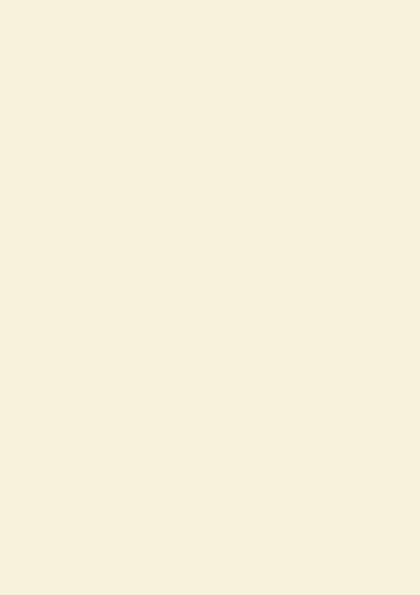
\includegraphics{空白示例.png}, center, scale=1, angle=0, opacity=1}
\BgThispage

\subsection{对象}
正如 Java 一样,C++ 的对象也是类的具体化。建立一个对象的格式同样也是
\begin{quote}
  \verb!Person p;!
\end{quote}
而访问一个对象的成员的格式同样也是
\begin{quote}
  \verb!p.age! \qquad \verb!p.show()!
\end{quote}

但与 Java 不同的是,C++ 有指针。在下面的例子中,定义一个指针变量 $q$,其指向对象 $p$ 的地址,写成 \verb!Person *q = &p!。此时要访问 $q$ 的成员,则需要以箭头 (\verb!->!) 替代点号 (\verb!.!) 以完成指针操作。

\begin{lstlisting}
#include<stdio.h>
#include<string.h>

class Person{
	private:
		char name[30];
		int age;
	public:
		Person(char newName[30], int newAge);
		void show();
};
Person::Person(char newName[30], int newAge){ //Person构造器的定义
	strcpy(this->name, newName);
	this->age = newAge;
}
void Person::show(){  //show()函数的定义
	printf("name: %s, age: %d\n", this->name, this->age);
}
int main(){
	Person p = Person("XiaoMing", 19);
	Person *q = &p;
	q->show();
}
\end{lstlisting}

此外,C++ 也存在 \keyword{this} 关键字。通过构造器构造对象时,它同样指向这个对象的地址。

关于变量的初始值:
\begin{itemize}[itemsep=0pt,parsep=0pt]
    \item 使用 \keyword{static} 修饰的静态成员变量的初值为 0。
    \item 如果对象是全局的、静态的,那它成员的初值就是 0。
    \item 如果既不是静态对象,也不是静态成员变量,那初值不确定。
\end{itemize}

\subsection{构造函数}
构造函数用于构造一个新的对象。构造函数不设返回值,可以重载,放在类的内部或者外部定义都可以。如果没有显式定义构造函数,系统也会默认指定一个空的构造函数;但只要显式定义了,那就不会指定空构造函数了(除非再写一个来重载)。

在主函数中,要分清构造的语法。
\begin{itemize}
  \item Java:\verb!Person p = new Person("XiaoMing", 19);!
  \item C++:\verb!Person p = Person("XiaoMing",19);! 或 \verb!Person p("XiaoMing",19);!
\end{itemize}

以下的例子中,提供了三个构造器的重载。
\begin{lstlisting}
#include<stdio.h>
#include<string.h>

class Person{
	private:
		char name[30];
		int age;
	public:
		Person();
		Person(int x);
		Person(char *newName, int newAge);
		void show();
};
Person::Person(){ //空参数构造器
	strcpy(this->name, "佚名");
	this->age = 0;
}
Person::Person(int x){ //单一参数的构造器(int)
	strcpy(this->name, "佚名");
	this->age = x;
}
Person::Person(char *newName, int newAge){ //双参数构造器(char*, int)
	strcpy(this->name, newName);
	this->age = newAge;
}
void Person::show(){
	printf("name: %s, age: %d\n", this->name, this->age);
}

int main(){
	Person p1("XiaoMing", 19);
	Person p2(20);
	Person p3; //值得一提的是,使用无参数构造器不用加空括号"()"
	p1.show(); p2.show(); p3.show();
}
\end{lstlisting}

还可以使用初始化表,对成员批量初始化。

\paragraph{拷贝构造函数} 「拷贝构造函数」是构造函数的一种,它代表把一个对象的所有值复制给另一个对象。如果没有拷贝构造函数,那系统会默认提供一个成员逐个复制的构造函数,这是一种「浅复制」。如果写了拷贝构造函数,那就可以用它实现「深复制」。

\begin{lstlisting}
    Person (Person &p){ //这就是拷贝构造函数的格式例子
        strcpy(this->name, p.name);
        this->age = p.age;
    }
\end{lstlisting}

\paragraph{析构函数} 「析构函数」是对象生命期结束后系统自动调用的一种函数,通常用于回收资源。其名称即为类名前加上波浪号 (\verb!~!),无参数,无返回值,不可重载。若没有析构函数,则系统会自动提供一个空的析构函数,有点类似Java里类的 \verb!finalize! 方法。就像这样:

\begin{lstlisting}
    ~Person(){
		printf("执行析构函数"); //函数体,例子是示意性的,一般在这里回收资源
	}
\end{lstlisting}

那么创建的 \verb!Person! 类实例会在其生命期结束之后调用这个函数。

\section{类与对象·进阶}
\subsection{对象与类的那些琐事儿}
\paragraph{动态分配内存} 在 C++ 中,用 \keyword{new} 和 \keyword{delete} 可以动态分配内存,不过使用的方法与 Java 的 \keyword{new} 有所不同。

\paragraph{对象数组} 对象数组则是元素为一个个对象的数组。比如
\begin{itemize}[itemsep=0pt,parsep=0pt]
  \item C++:\verb!Person p[5];!
  \item Java:\verb!Person [] p = new Person[5];!
\end{itemize}

\paragraph{消歧义} 类有其作用域。如果出现了同名的局部变量与成员变量,那么可以用 \verb!类名::变量名! 的方法加以界定(Java 是\verb!类名.变量名!)。

\paragraph{对象作成员} 一个类的成员除了可以是 \keyword{int}、\keyword{char} 等基本数据类型以外,还可以是别的类的对象。这点在 Java 自然也是一样的。

\subsection{常成员和静态成员}
\paragraph{常成员函数} 这是一种使用 \keyword{const} 定义的成员函数。它可以读取其中成员的值但不能修改它,也不能调用其他的非「常成员函数」。

在 Java 中,类似于 \keyword{final} 修饰的成员函数。

\paragraph{常对象} 这是一种使用 \keyword{const} 修饰的对象。它在定义时应该被初始化,而且在整个生存期内不能被修改。

有点像 Java 中的「终稿类」(\keyword{final} 修饰)。

\paragraph{静态成员} 这是一种使用 \keyword{static} 修饰的成员变量或成员函数。其中,\verb!public! 修饰的静态成员可以直接用类名来访问。

在 Java 中,与下面的方式类似:
\begin{tcolorbox}[colback=cyan!10, colframe=cyan, arc=1pt]
    对于成员变量,以下的访问是允许的:
    \begin{itemize}[itemsep=0pt,parsep=0pt]
        \item \verb!实例.实例变量!——\verb!p.name!
        \item \verb!实例.类变量!——\verb!p.age!
        \item \verb!类.类变量!——\verb!Person.age!
    \end{itemize}
    (实例变量=动态变量,类变量=静态变量= \keyword{static} 修饰的变量,参见「知识小料」·其三十一第 3,4 页)
\end{tcolorbox}

值得一提的是:静态成员函数中不可以访问非静态成员!这在 Java 中也是一致的——\Emph{静态方法中不可以访问非静态成员!}我们称之为「静不容动」。

\subsection{友元}
\paragraph{友元函数} 友元函数是一种能够直接访问到类的 \keyword{private} 成员的一种函数,在声明时使用 \keyword{friend} 关键字修饰。

\begin{lstlisting}
#include<stdio.h>
#include<string.h>

class Person{
	private:
		char* name;
		int age;
	public:
		Person(char *newName, int newAge){
			name = new char[strlen(newName)+1];
			strcpy(this->name, newName);
			this->age = newAge;
		}
		friend void show(Person &p){ //通过友元函数能直接访问私有成员name和age
			printf("name:%s, age:%d\n", p.name, p.age);
		}
};
int main(){
	Person p("小明",19);
	show(p); //调用这个友元函数
}
\end{lstlisting}

\paragraph{友元类} 如果甲类被声明为乙类的友元类,那么甲类就可以访问乙类的全部成员。相当于打破了访问控制符的框架。

\section{继承(只列出基础部分)}
C++ 和 Java 一样也有继承的概念。

\begin{itemize}[itemsep=0pt,parsep=0pt]
  \item 父类=基类,子类=派生类。
  \item C++\Emph{能够多重继承}:一个子类能继承多个父类。
  \item 继承方式分 \verb!public!>\verb!protected!>\verb!private! 三种,父类的 \verb!public!和\verb!protected! 成员按照「降级至继承方式,只降不升」的规则继承到子类。
  \item 子类的构造函数总会调用父类的构造函数,这与 Java 类似,只不过 C++ 没有 \verb!super! 这一关键字。
  \item 子类的析构函数总会调用父类的析构函数。
  \item 子类函数可以重写(Override)父类的函数。
  \item 对于多继承,子类需要调用所有父类的构造函数。
  \item 了解:多重继承的二义性、赋值兼容规则、虚函数、抽象类。
\end{itemize}

以下的例子中,子类 Circle 继承了父类 Shape,且子类的构造函数调用了父类的构造函数。
\begin{lstlisting}
#include<stdio.h>
#include<string.h>

class Shape{ //父类:形状
	protected:
		char color;
		int x,y;
	public:
		Shape(){}
		Shape(char color, int x, int y){ //父类的构造函数
			this->x = x;
			this->y = y;
			this->color = color;
		}
};

class Circle : public Shape{ //子类:圆形,继承方式为公有
    //相当于子类取得了父类的成员color,x,y,而且取protected为新访问控制类型(protected遇到public只降不升,保持protected不变)
	private:
		int r;
	public:
		Circle(){}
		Circle(char color,int x,int y,int r) : Shape(color, x, y){
			//子类的构造函数,调用了父类的构造函数Shape(color,x,y)
			this->r = r;
		}
		void show(){
			printf("color:%c, (x,y)=(%d,%d), r=%d\n", color,x,y,r);
		}
};

int main(){
	Circle c = Circle('R', 1,2,3);
	c.show();
}
\end{lstlisting}

\section{模板}
模板相当于 Java 的「泛型」,意为通过一个「模具」能够生成不同的函数、类。

\subsection{函数模板}
通过函数模板,可以生成多个类似的函数。比如说,对于求最大值的\verb!max!函数,我们希望它的两个参数无论是\verb!int!、\verb!char!、\verb!double!等,函数都可以工作,那么可以写成模板的形式:
\begin{lstlisting}
template<class T>  //T泛指各种数据类型
T max(T a, T b){
    return (a>=b) ? a : b;
}
\end{lstlisting}

那么在主函数中,像 \verb!max(3,5)!、\verb!max('A','a')!、\verb!max(10.1, 12.3)! 这样的调用方式,无论参数是 \verb!int!、\verb!char!、\verb!double!,只要两个参数是同型的,就可以自由地使用这个模板。

事实上,当调用 \verb!max(3,5)! 时,编译器就会像作填空一样,把 \verb!int! 填入 \verb!T! 的位置,根据函数模板自动生成一个下面的「模板函数」。
\begin{quote}
  \verb!int max(int a,int b) { return (a>=b) ? a : b;}!
\end{quote}
这就是模板的「实例化」。

有时模板需要接收一些非类型参数,那么在调用的时候需要以常量来作实参。

\begin{lstlisting}
#include<stdio.h>
#include<string.h>

template<class T, int n> //模板中的n为非类型参数
void init(T *a, T b){
    for(int i=0; i<n; i++) a[i] = b;
}

int main(){
	int a[5];
	init <int,4> (a, 3); //注意配一对尖括号,写上填入模板的具体类型,且非类型参数n必须填常数
	for(int i=0; i<5; i++){
		printf("a[%d] = %d\n", i, a[i]);
	}
	//这个程序的功能是,将a数组的前4个元素赋值为3。
}
\end{lstlisting}


\subsection{类模板}
通过类模板,可以生成多个相似的类。

因此经由类模板产生对象,需要两个步骤:$\text{类模板}\xrightarrow{\text{实例化}}\text{类}\xrightarrow{\text{实例化}} \text{对象}$。

\subsection{Java 泛型例子}
相信大家对Java的「泛型」还是感到陌生,这里举一个泛型的例子,返回两个任意类的最大值。其中需要调用 \verb!Comparable! 接口,对对象使用 \verb!compareTo! 方法实现。



\begin{lstlisting}[language=Java]
public class Test {
	//泛型方法返回两个数的最大值
	public static <T extends Comparable<T> > T max(T a, T b) {
		return (a.compareTo(b) > 0) ? a : b;
	}
	public static void main(String args[])
    {
        System.out.println(max(3, 5));
        System.out.println(max('A', 'a')); //A=65, a=97
        System.out.println(max(10.1, 12.3));
    }
}
\end{lstlisting}

\section{运算符重载}
这一段内容是 C++ 特有的。

有时我们希望一种运算可以用于自定义的类,比如复数类可以用 \verb!c=a.add(b)! 这样的语句实现加法,但是写成 \verb!c=a+b! 更有美感,那么这就是「加号(\verb!+!)的重载」——把加号看成函数,两个加数是函数的参数。

\begin{itemize}[itemsep=0pt,parsep=0pt]
  \item 运算符重载本质上是函数的重载。
  \item 重载运算符通常被声明为类的成员函数或友元函数,这样便于访问 \keyword{private} 成员。
  \item 有些运算符不能重载。
  \item 关于参数个数——对于$n$目运算符,重载为成员函数对应 $n-1$ 个形参,而重载为友元函数对应 $n$ 个形参。
\end{itemize}

以下的例子中,实现了复数加法的重载,其中重载为类的成员函数。
\begin{lstlisting}
#include<stdio.h>
#include<string.h>
class Complex{
	private:
		int r,i; //复数类的实部与虚部
	public:
		Complex(int r, int i){ //构造器
			this->r = r;
			this->i = i;
		}
		void show(){printf("%d + %di\n", r, i);}
		Complex operator+(Complex &c){ //重载加号运算符函数
			Complex sum(0,0); //定义局部变量时需要初始化
			sum.r = this->r + c.r;
			sum.i = this->i + c.i;
			return sum;
		}
};

int main(){
	Complex c1(3,4), c2(-1,5);
	Complex c3 = c1 + c2; //调用重载的加法运算函数
	c3.show();
}
\end{lstlisting}

\backgroundsetup{contents=
\includegraphics{下半示例.png}, center, scale=1, angle=0, opacity=1}
\BgThispage

\end{document} 